\documentclass[aspectratio=169,9pt]{beamer}
\usepackage[utf8]{inputenc}
\usepackage[T1]{fontenc}
\usepackage[brazilian]{babel}
\usepackage{tgheros}
\renewcommand{\familydefault}{\sfdefault}
\usepackage{booktabs}
\usepackage{array}
\usepackage{amsmath}
\usepackage{tikz}
\usetikzlibrary{arrows.meta,positioning,decorations.pathreplacing}

\usetheme{default}
\usecolortheme{default}
\setbeamertemplate{navigation symbols}{}

\definecolor{navy}{RGB}{18,34,56}
\definecolor{navy2}{RGB}{31,58,86}
\definecolor{gold}{RGB}{176,141,63}
\definecolor{lightbg}{RGB}{244,243,239}
\definecolor{softgray}{RGB}{110,110,110}

\setbeamertemplate{footline}{%
  \hspace{0.35cm}\raisebox{2pt}{\tiny\color{softgray} AAET \hspace{0.5em}\textbullet\hspace{0.5em} PONTO CEGO}%
  \hfill\raisebox{2pt}{\tiny\color{softgray}\insertframenumber\,/\,\inserttotalframenumber}\hspace{0.35cm}\vspace{2pt}}
\setbeamercolor{frametitle}{fg=white,bg=navy}
\setbeamercolor{title}{fg=white,bg=navy}
\setbeamerfont{frametitle}{series=\bfseries,size=\large}
\setbeamertemplate{frametitle}{%
  \vskip-1pt\hspace{-1pt}%
  \begin{beamercolorbox}[wd=\paperwidth,sep=7pt,leftskip=10pt]{frametitle}
    \usebeamerfont{frametitle}\insertframetitle
    \hfill{\small\color{gold}\insertframesubtitle}
  \end{beamercolorbox}}
\setbeamertemplate{itemize items}{\raisebox{0.6pt}{\tiny\color{gold}$\blacktriangleright$}}
\setlength{\parskip}{2pt}
\let\olditem\item
\renewcommand\item{\olditem\vspace{0.5pt}}

\newcommand{\crit}[1]{{\scriptsize\color{gold}\textbf{#1}}}
\newcommand{\sechead}[1]{{\bfseries\color{navy}#1}}

\title{}
\author{}
\date{}

\begin{document}

% ============================================================
% PAGE 1 -- ROBO + TESE
% ============================================================
\begin{frame}[plain]
\begin{tikzpicture}[remember picture, overlay]
\fill[navy] (current page.north west) rectangle ([yshift=-2.35cm]current page.north east);
\node[anchor=west, text=white] at ([xshift=0.55cm,yshift=-1.15cm]current page.north west)
  {\fontsize{30}{30}\selectfont\bfseries PONTO CEGO};
\node[anchor=west, text=gold] at ([xshift=0.6cm,yshift=-1.95cm]current page.north west)
  {\small Reversão de preço na lacuna de monitoramento institucional};
\node[anchor=east, text=white] at ([xshift=-0.55cm,yshift=-1.5cm]current page.north east)
  {\footnotesize\begin{tabular}{r} AAET \\[-1pt] \footnotesize\color{gold} Carta de estratégia \end{tabular}};
\end{tikzpicture}

\vspace{2.5cm}
\footnotesize
\begin{columns}[T]
\begin{column}{0.5\textwidth}
\crit{APRESENTAÇÃO DO ROBÔ}\\[2pt]
\textbf{\sechead{Por que ``Ponto Cego''.}} Ações pouco monitoradas por fundos
não têm quem corrija um exagero de preço rapidamente -- é o ponto cego do
mercado institucional. O robô compra exatamente aí, e espera 3 meses para
agir: é o tempo real que o mercado leva para \emph{enxergar} esse ponto cego,
já que a CVM divulga a carteira dos fundos com $\sim$90 dias de defasagem. O
nome descreve o quê (região sem vigilância) e o como (a defasagem que define
o horizonte).

\vspace{5pt}
\crit{CONCEITO -- TESE CENTRAL}\\[2pt]
\textbf{\sechead{Ineficiência.}} Reversão de curto prazo (Jegadeesh, 1990) só
existe onde faltam agentes sofisticados para arbitrar o exagero --
\emph{limits-to-arbitrage} (Shleifer \& Vishny, 1997). Usamos presença
institucional (Seção seguinte) como termômetro direto de quem vigia cada ação.
\end{column}
\begin{column}{0.5\textwidth}
\begin{tikzpicture}[scale=1, every node/.style={font=\scriptsize}]
\draw[fill=lightbg, draw=navy!30, rounded corners] (0,0) rectangle (6.3,5.3);
\node[navy, font=\bfseries\small] at (3.15,4.85) {O mecanismo, em 4 passos};
\foreach \i/\txt/\y in {
  1/{Ação sobe ou cai forte num mês}/3.95,
  2/{Poucos fundos a monitoram (baixa presença institucional)}/3.1,
  3/{Ninguém arbitra o exagero -- ele persiste}/2.25,
  4/{3 meses depois (defasagem real de dado CVM) o preço reverte}/1.35} {
  \node[circle, fill=gold, text=white, font=\bfseries\tiny, minimum size=15pt, inner sep=0pt] at (0.65,\y) {\i};
  \node[align=left, text width=5.2cm, anchor=west] at (1.15,\y) {\txt};
}
\node[align=center, text=navy, font=\bfseries\scriptsize] at (3.15,0.5) {Compra: perdedores recentes\\em baixa presença $\;\vert\;$ Venda: vencedores};
\end{tikzpicture}
\end{column}
\end{columns}
\end{frame}

% ============================================================
% PAGE 2 -- BASE CONSOLIDADA (LOOK-THROUGH) -- diferencial criativo
% ============================================================
\begin{frame}{A base}{Consolidação look-through}
\crit{CONCEITO -- O QUE TORNA ESSE SINAL DIFERENTE}

\vspace{2pt}
A maioria das análises de posse institucional no Brasil usa a carteira
\textbf{direta} dos fundos (CDA/CVM). Isso subestima -- às vezes
dramaticamente -- a presença institucional real, porque ignora fundos que
investem em outros fundos (FIC). Nossa base é \textbf{consolidada
(look-through)}: reconstruímos a exposição efetiva de cada fundo a cada ação,
atravessando cadeias de fundo-de-fundos em até \textbf{20 níveis de
profundidade}, para o universo completo de fundos brasileiros, 2016--2026.

\vspace{2pt}
\begin{tikzpicture}[every node/.style={font=\scriptsize}]
\node[draw=navy, fill=navy!6, rounded corners, minimum width=2.5cm, minimum height=0.8cm, align=center] (A) at (0,0) {Fundo A\\\footnotesize\textit{multimercado}};
\node[draw=navy, fill=navy!6, rounded corners, minimum width=2.5cm, minimum height=0.8cm, align=center] (B) at (3.9,0) {Fundo B\\\footnotesize\textit{FIC}};
\node[draw=gold, fill=gold!12, rounded corners, minimum width=2.5cm, minimum height=0.8cm, align=center] (X) at (7.8,0) {Ação X\\\footnotesize\textit{ex.: VALE3}};
\draw[-{Latex}, navy] (A) -- (B) node[midway, above, font=\tiny] {30\% das cotas};
\draw[-{Latex}, navy] (B) -- (X) node[midway, above, font=\tiny] {5\% da carteira};
\node[align=left, text width=3.2cm, font=\scriptsize, text=softgray] at (0,-1.1) {Base direta (CDA ingênua):\\\textbf{\color{softgray}A não aparece em X}};
\node[align=left, text width=4.6cm, font=\scriptsize, text=navy] at (5.85,-1.1) {Base PONTO CEGO (consolidada):\\\textbf{\color{navy}A tem 1,5\% de exposição efetiva a X} (via B)};
\end{tikzpicture}

\vspace{6pt}
\begin{columns}[T]
\begin{column}{0.5\textwidth}
\footnotesize\textbf{\sechead{Fórmula (recursiva, até nível 20):}}
\[
E^{\text{cons}}_{f,i} = E^{\text{direta}}_{f,i} +\!\!\sum_{g\,\in\,\text{cotas de }f}\!\! \omega_{f\to g}\cdot E^{\text{cons}}_{g,i}
\]
\[
\omega_{f\to g} = \dfrac{\text{Valor de }f\text{ em cotas de }g}{\text{PL de }g}
\]
\end{column}
\begin{column}{0.5\textwidth}
\footnotesize\textbf{\sechead{Por que importa aqui:}} nosso ranking de
``presença institucional'' (base do sinal, Seção seguinte) é medido sobre
$E^{\text{cons}}$, não posse direta -- classifica corretamente ações que
\emph{parecem} desmonitoradas mas têm exposição institucional oculta via FIC,
e vice-versa.
\end{column}
\end{columns}
\end{frame}

% ============================================================
% PAGE 3 -- MODELAGEM
% ============================================================
\begin{frame}{Modelagem}{Dados, sinal e teste}
\begin{columns}[T]
\begin{column}{0.34\textwidth}
\crit{DADOS DE ENTRADA}
\begin{itemize}
\item Retorno mensal de cada ação (2016--2026)
\item Exposição \textbf{consolidada} ($E^{\text{cons}}$) do universo de fundos
  brasileiros a cada ação-mês
\end{itemize}
\crit{SINAL}
\[
\text{Presença}_{i,t} = \text{pctl}_t\Big(\textstyle\sum_f E^{\text{cons}}_{f,i,t}\Big)
\]
\[
s_{i,t} = r_{i,t-1} \;\Big|\; \text{Presença}_{i,t}\le p_{33}
\]
\end{column}
\begin{column}{0.34\textwidth}
\crit{DECISÃO}
\begin{itemize}
\item Terço de menor presença institucional
\item Dentro dele, quintis por $s_{i,t}$
\item \textbf{Compra}: Q1 (perdedores) \quad\textbf{Venda}: Q5 (vencedores)
\item Rebalanceamento mensal, holding de 3 meses
\end{itemize}
\crit{TESTE (mesma régua p/ todos candidatos)}
\[
r_{i,t+3} = \alpha_t + \beta_t\, s_{i,t} + \varepsilon_{i,t} \;\; \text{(mês a mês)}
\]
\[
\hat t_{\text{NW}} = \bar\beta \,/\, \text{se}_{\text{Newey--West}}(\bar\beta)
\]
\end{column}
\begin{column}{0.32\textwidth}
\begin{center}
\scriptsize
\begin{tabular}{lccc}
\toprule
Amostra & $n$m & $t_{\text{NW}}$ & $p$ \\
\midrule
\textbf{Baixa presença} & 60 & $\mathbf{-2{,}22}$ & $\mathbf{0{,}031}$ \\
Alta presença & 59 & $-0{,}91$ & $0{,}366$ \\
Sem filtro & 60 & $-1{,}77$ & $0{,}083$ \\
\bottomrule
\end{tabular}
\end{center}
\vspace{4pt}
\footnotesize O efeito só existe na baixa presença -- padrão diferencial que
sustenta a tese, não é ruído de uma busca isolada.

\vspace{4pt}
\footnotesize\textbf{Sistemático}: cortes de quintil e universo de baixa
presença estimados só no treino (antes de 2020); regra 100\% mecânica.
\end{column}
\end{columns}
\end{frame}

% ============================================================
% PAGE 4 -- BACKTEST
% ============================================================
\begin{frame}{Backtest}{Desenho, vieses e performance}
\begin{columns}[T]
\begin{column}{0.30\textwidth}
\crit{DESENHO}
\begin{itemize}
\item Fora da amostra: fev/2020--jun/2026 (60 meses); cortes fixados só no
  treino pré-2020
\item Peso igual por perna, rebalanceamento mensal
\item Benchmark: Ibovespa, mesmo período exato
\end{itemize}
\crit{VIESES MITIGADOS}
\begin{itemize}
\item Sem look-ahead (cortes nunca veem teste)
\item $h=3$ fixado \emph{a priori} pela defasagem real do dado
\item Mesma régua estatística usada p/ \textbf{descartar} 2 outros
  candidatos (fluxo entre fundos; HHI) -- Seção seguinte
\end{itemize}
\end{column}
\begin{column}{0.70\textwidth}
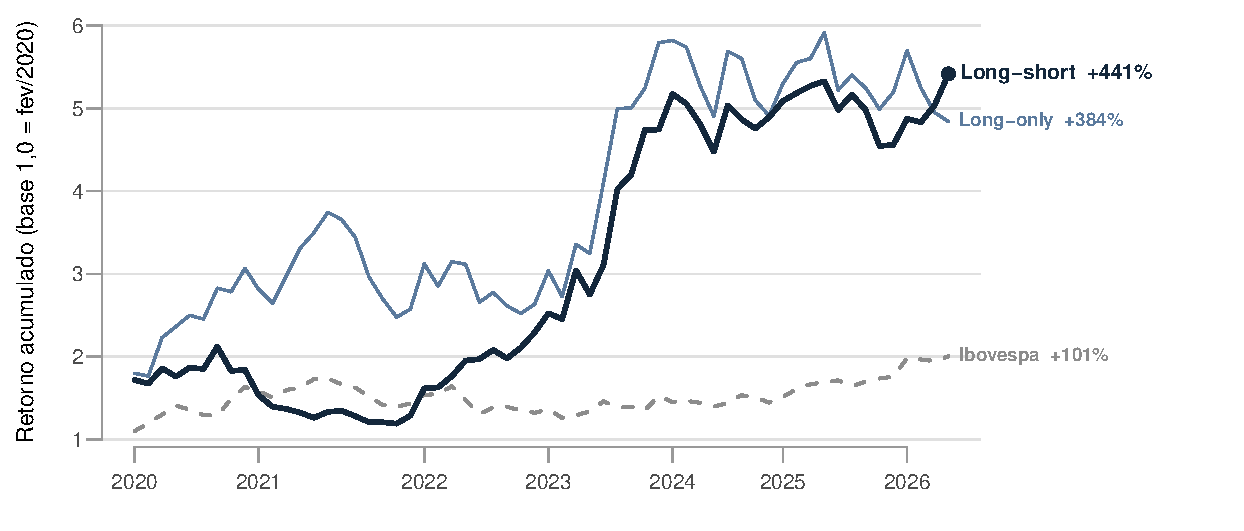
\includegraphics[width=\textwidth]{fig_equity.pdf}
\vspace{2pt}
\begin{center}
\scriptsize
\begin{tabular}{lccc}
\toprule
 & Long-short & Long-only & Ibovespa \\
\midrule
Retorno anualizado & $50{,}8\%$ & $50{,}3\%$ & $17{,}1\%$ \\
\textbf{Sharpe anualizado} & $\mathbf{0{,}96}$ & $0{,}85$ & $0{,}80$ \\
Max drawdown & $43{,}8\%$ & $33{,}8\%$ & $27{,}4\%$ \\
\bottomrule
\end{tabular}
\hspace{8pt}
\parbox{5.5cm}{\scriptsize\raggedright Alfa mensal (long-short vs. Ibov)
$=3{,}10\%$ ($p{=}0{,}067$); beta $=0{,}29$ (n.s.) -- sem custo de
transação/liquidez, limitação assumida na Seção seguinte.}
\end{center}
\end{column}
\end{columns}
\end{frame}

% ============================================================
% PAGE 5 -- ANALISE + CONCLUSAO + IA
% ============================================================
\begin{frame}{Análise, conclusão \& IA generativa}{}
\begin{columns}[T]
\begin{column}{0.5\textwidth}
\crit{ANÁLISE DOS RESULTADOS}
\begin{itemize}
\item Sharpe (0,96) supera o Ibovespa (0,80), mas drawdown (44\%) também é
  maior -- esperado em ações pequenas e menos líquidas, onde o sinal existe
\item Alfa mensal positivo, $p=0{,}067$ isolado (60 obs): marginal, mas
  consistente com o Fama--MacBeth já validado
\item \textbf{Limitações}: sem custo de transação/liquidez (perna comprada em
  small caps); cobertura de preço incompleta pré-2022 p/ tickers
  descontinuados; teste único, sem correção formal de múltiplas comparações
\end{itemize}
\crit{CONCLUSÃO \& PRÓXIMOS PASSOS}
\begin{itemize}
\item Sinal robusto, não livre de dúvida. Próximos passos: custo de
  transação/liquidez explícitos; sizing por vol. inversa (reduz drawdown);
  validar defasagem de divulgação fundo a fundo (não é uniforme)
\end{itemize}
\end{column}
\begin{column}{0.5\textwidth}
\crit{USO DE IA GENERATIVA}\\[2pt]
\footnotesize Claude (Anthropic) foi usado em todas as etapas -- distinção
entre trabalho da equipe e contribuição da IA:
\begin{itemize}
\item \textbf{Dados} (equipe define, IA executa): reconstrução da base
  consolidada CVM 2016--2026 e correção de 4 inconsistências reais na fonte
  (formato numérico, estabilidade de ID de fundo, subclasses pós-reforma
  CVM175)
\item \textbf{Hipóteses} (IA gera, equipe julga): 10+ sinais formulados e
  testados com a mesma régua -- 2 candidatos com aparência forte foram
  \textbf{descartados} por não sobreviverem a Newey--West, disciplina que a
  IA aplicou de forma consistente a cada um
\item \textbf{Backtest/código}: implementação de Fama--MacBeth, Newey--West
  e simulação de portfólio, com verificação numérica em cada etapa
\item \textbf{Limitação encontrada}: IA não substitui julgamento sobre
  quais candidatos são economicamente plausíveis -- esse crivo permaneceu
  humano em cada decisão de descarte
\end{itemize}
\end{column}
\end{columns}
\end{frame}

\end{document}
